
\documentclass[11pt,letterpaper]{article}

% ---------------------------------------------------------
% Paquetes
% ---------------------------------------------------------

\usepackage[utf8]{inputenc}
\usepackage[T1]{fontenc}
\usepackage[spanish]{babel}
\usepackage{graphicx}
\usepackage{geometry}
\usepackage{amsmath}
\usepackage{amssymb}
\usepackage{listings}
\usepackage{xcolor}
\usepackage{float}
\usepackage{booktabs}
\usepackage[hidelinks]{hyperref}

\geometry{letterpaper, margin=2.1cm}

% ---------------------------------------------------------
% Configuración del código Python
% ---------------------------------------------------------

\lstset{
    language=Python,
    basicstyle=\ttfamily\footnotesize,
    keywordstyle=\color{blue},
    commentstyle=\color{gray},
    stringstyle=\color{red!60!black},
    numbers=left,
    numberstyle=\tiny,
    frame=single,
    breaklines=true,
    showstringspaces=false,
    columns=fullflexible,
    keepspaces=true
}

% ---------------------------------------------------------
% Datos
% ---------------------------------------------------------

\title{
    Taller 7: Filtrado de Imágenes\\
    en el Dominio de la Frecuencia
}

\author{
    Camilo Eduardo Muñoz Albornoz\\
    Procesamiento Digital de Imágenes\\
    Universidad Tecnológica de Pereira
}

\date{}

\begin{document}

\maketitle

\begin{center}

\textbf{Código fuente en GitHub}\\[0.2cm]

\textbf{Carpeta del Taller 7: }
\href
{https://github.com/CamiloMunozAL/ProcDImagenes/tree/main/taller7}
{\textcolor{blue}{
\underline{
\texttt{github.com/CamiloMunozAL/ProcDImagenes/tree/main/taller7}
}
}}

\vspace{0.2cm}

\textbf{Cuaderno Python: }
\href
{https://github.com/CamiloMunozAL/ProcDImagenes/blob/main/taller7/taller7.ipynb}
{\textcolor{blue}{
\underline{\texttt{taller7.ipynb}}
}}

\end{center}

% =========================================================
\begin{abstract}

En este taller se implementaron seis filtros en el
dominio de la frecuencia: ideal, Butterworth y Gaussiano,
en sus versiones paso bajo y paso alto.

Los algoritmos se desarrollaron en Python utilizando
ciclos para construir las máscaras de frecuencia y la
Transformada Rápida de Fourier (FFT) para transformar
y reconstruir las imágenes.

Las pruebas se realizaron con tres imágenes en escala
de grises: un cuadrado blanco sobre fondo negro,
un rostro y un paisaje natural. Se utilizaron
frecuencias de corte de 20, 40 y 80, además de
diferentes órdenes para los filtros Butterworth.

Los resultados permitieron observar cómo los filtros
paso bajo suavizan las imágenes, mientras que los
paso alto resaltan bordes y variaciones rápidas
de intensidad. También se analizaron los efectos
de anillado producidos por las transiciones
abruptas entre frecuencias.

\end{abstract}

% =========================================================
\section{Objetivos}

\begin{enumerate}

    \item Implementar mediante ciclos un filtro ideal
    paso bajo en 2D que reciba una imagen y una
    frecuencia de corte.

    \item Implementar un filtro Butterworth paso bajo
    en 2D, utilizando la frecuencia de corte y el
    orden como parámetros.

    \item Implementar mediante ciclos un filtro
    Gaussiano paso bajo en 2D para diferentes
    frecuencias de corte.

    \item Implementar un filtro ideal paso alto
    en 2D que permita destacar las variaciones
    rápidas de intensidad.

    \item Implementar un filtro Butterworth paso alto
    en 2D y analizar el efecto de la frecuencia
    de corte y del orden.

    \item Implementar un filtro Gaussiano paso alto
    en 2D y observar su comportamiento sobre
    bordes y texturas.

\end{enumerate}

% =========================================================
\section{Fundamentos teóricos}

\subsection{Filtrado en el dominio de la frecuencia}

Una imagen digital puede representarse en el dominio
espacial mediante una matriz de intensidades, donde
cada elemento corresponde a un píxel.

Sin embargo, también puede representarse en el
dominio de la frecuencia mediante la Transformada
de Fourier.

En este dominio, la imagen se describe a partir
de componentes asociadas con diferentes velocidades
de cambio de intensidad.

Las frecuencias bajas se relacionan principalmente
con variaciones graduales y estructuras amplias,
mientras que las frecuencias altas se relacionan
con detalles finos, texturas y cambios bruscos.

El filtrado en frecuencia consiste en modificar
estas componentes mediante una función
$H(u,v)$, denominada máscara o función
de transferencia del filtro.

El procedimiento general es:

\begin{enumerate}

    \item Transformar la imagen al dominio
    de la frecuencia.

    \item Multiplicar su transformada por
    la máscara del filtro.

    \item Aplicar la transformada inversa
    para recuperar la imagen procesada.

\end{enumerate}

Matemáticamente:

\begin{equation}
G(u,v)=F(u,v)H(u,v)
\label{eq:filtrado}
\end{equation}

Donde:

\begin{itemize}

    \item $F(u,v)$ es la transformada de Fourier
    de la imagen original.

    \item $H(u,v)$ es la máscara del filtro.

    \item $G(u,v)$ es la transformada
    de la imagen filtrada.

\end{itemize}

Finalmente, se utiliza la transformada inversa
de Fourier para regresar al dominio espacial.

\subsection{Frecuencia de corte}

La frecuencia de corte, representada por $D_0$,
es un parámetro que determina la región del
espectro que se conserva o atenúa.

Para calcular la distancia desde una posición
$(u,v)$ hasta el centro del espectro se utiliza:

\begin{equation}
D(u,v)=
\sqrt{
(u-u_c)^2+(v-v_c)^2
}
\end{equation}

Donde $(u_c,v_c)$ representa el centro
de la transformada.

En este trabajo se utilizó
\texttt{fftshift()} para colocar la
frecuencia cero en el centro.

\subsection{Filtros paso bajo}

Los filtros paso bajo conservan principalmente
las frecuencias bajas y atenúan las altas.

Como resultado, disminuyen los cambios rápidos
de intensidad y producen suavizado.

En general, una frecuencia de corte pequeña
genera mayor desenfoque, mientras que una
frecuencia de corte grande permite conservar
más detalles.

\subsection{Filtros paso alto}

Los filtros paso alto realizan la operación
contraria: atenúan las frecuencias bajas
y conservan las altas.

Esto permite resaltar bordes, texturas
y otras variaciones rápidas de intensidad.

Las máscaras paso alto pueden obtenerse
a partir de las correspondientes máscaras
paso bajo:

\begin{equation}
H_{HP}(u,v)=1-H_{LP}(u,v)
\label{eq:complemento}
\end{equation}

Al eliminar la componente continua,
los resultados suelen contener valores
positivos y negativos alrededor de cero.

Por esta razón, para las visualizaciones
se utilizó la magnitud absoluta de las
respuestas, manteniendo una escala
común entre 0 y 255.

% =========================================================
\section{Imágenes y metodología}

\subsection{Imágenes utilizadas}

Para evaluar los filtros se seleccionaron
tres imágenes en escala de grises con
características diferentes.

\begin{itemize}

    \item \textbf{Cuadrado:}
    imagen sintética de $256\times256$ píxeles,
    con un cuadrado blanco de $128\times128$
    sobre fondo negro. Permite observar
    fácilmente el suavizado, los bordes
    y posibles oscilaciones.

    \item \textbf{Rostro:}
    fotografía con textura visible en la piel,
    ojos, cabello y contornos faciales.
    Se utilizó para observar la reducción
    de detalles y el comportamiento del
    filtrado sobre una fotografía.

    \item \textbf{Paisaje:}
    fotografía de montañas, árboles,
    vegetación y un lago con reflejos.
    Permite estudiar el efecto sobre
    estructuras naturales y texturas.

\end{itemize}

Las fotografías se cargaron en escala de grises
mediante OpenCV y conservaron sus dimensiones
originales. El cuadrado fue generado
directamente con NumPy.

Las imágenes y los resultados se visualizaron
mediante Matplotlib, utilizando una disposición
comparativa para facilitar su análisis.

\subsection{Preparación de los datos}

Se utilizaron las bibliotecas NumPy, OpenCV
y Matplotlib.

\begin{lstlisting}
import numpy as np
import cv2
import matplotlib.pyplot as plt

# Cuadrado sintetico
cuadrado = np.zeros(
    (256, 256),
    dtype=np.float64
)

cuadrado[64:192, 64:192] = 255

# Fotografias originales
rostro = cv2.imread(
    "images/rostro.png",
    cv2.IMREAD_GRAYSCALE
)

paisaje = cv2.imread(
    "images/paisaje.png",
    cv2.IMREAD_GRAYSCALE
)

if rostro is None or paisaje is None:
    raise FileNotFoundError(
        "No se encontraron las imagenes"
    )

imagenes = [
    cuadrado,
    rostro,
    paisaje
]

titulos = [
    "Cuadrado",
    "Rostro",
    "Paisaje"
]

frecuencias = [20, 40, 80]
\end{lstlisting}

Las mismas tres imágenes se utilizaron
en los seis ejercicios para mantener
condiciones de prueba consistentes.

Se eligieron frecuencias de corte
de 20, 40 y 80, según los valores
propuestos en el material del taller.

Debe considerarse que un mismo valor
de corte puede tener un efecto diferente
en imágenes de distintas dimensiones.

\subsection{Procedimiento común de filtrado}

Aunque los seis filtros tienen expresiones
matemáticas diferentes, en el código siguen
un patrón general común. Primero se calcula
la transformada de Fourier de la imagen y
se centra el espectro. Después se construye
la máscara correspondiente mediante ciclos,
se multiplica por la transformada centrada
y se aplica la transformada inversa para
regresar al dominio espacial.

La diferencia principal entre las funciones
está en la expresión utilizada para construir
la máscara $H(u,v)$: el filtro ideal utiliza
una condición sobre la distancia, Butterworth
utiliza la frecuencia de corte y el orden,
y el filtro Gaussiano utiliza una expresión
exponencial.

Este procedimiento representa el patrón general
que comparten las implementaciones del taller;
no se definió una función auxiliar independiente
para centralizarlo. Por ello, en los apartados
siguientes se presenta explícitamente el código
de cada filtro tal como fue implementado.

% =========================================================
\section{Desarrollo y resultados}

% ---------------------------------------------------------
\subsection{Punto 1: Filtro ideal paso bajo}

\subsubsection*{Objetivo}

Implementar un filtro ideal paso bajo en 2D
que reciba una imagen y una frecuencia de corte,
utilizando ciclos para construir la máscara.

\subsubsection*{Fundamento}

El filtro ideal paso bajo se define como:

\begin{equation}
H(u,v)=
\begin{cases}
1, & D(u,v)\leq D_0\\
0, & D(u,v)>D_0
\end{cases}
\end{equation}

La máscara conserva completamente las
frecuencias situadas dentro del radio
de corte y elimina las restantes.

Su transición es abrupta, por lo que
puede producir oscilaciones alrededor
de los bordes al reconstruir la imagen.

\subsubsection*{Implementación}

\begin{lstlisting}
def filtro_ideal_paso_bajo(imagen, frecuencia_corte):

    if frecuencia_corte <= 0:
        raise ValueError(
            "La frecuencia de corte debe ser positiva"
        )

    filas, columnas = imagen.shape

    mascara = np.zeros(
        (filas, columnas),
        dtype=np.float64
    )

    centro_fila = filas // 2
    centro_columna = columnas // 2

    for fila in range(filas):
        for columna in range(columnas):

            distancia = np.sqrt(
                (fila - centro_fila)**2
                + (columna - centro_columna)**2
            )

            if distancia <= frecuencia_corte:
                mascara[fila, columna] = 1

    transformada = np.fft.fft2(imagen)
    transformada_centrada = np.fft.fftshift(
        transformada
    )
    transformada_filtrada = (
        transformada_centrada * mascara
    )
    transformada_inversa = np.fft.ifftshift(
        transformada_filtrada
    )
    imagen_filtrada = np.fft.ifft2(
        transformada_inversa
    )
    resultado = np.real(imagen_filtrada)

    return resultado, mascara
\end{lstlisting}

\subsubsection*{Resultados y análisis}

\begin{figure}[H]
    \centering
    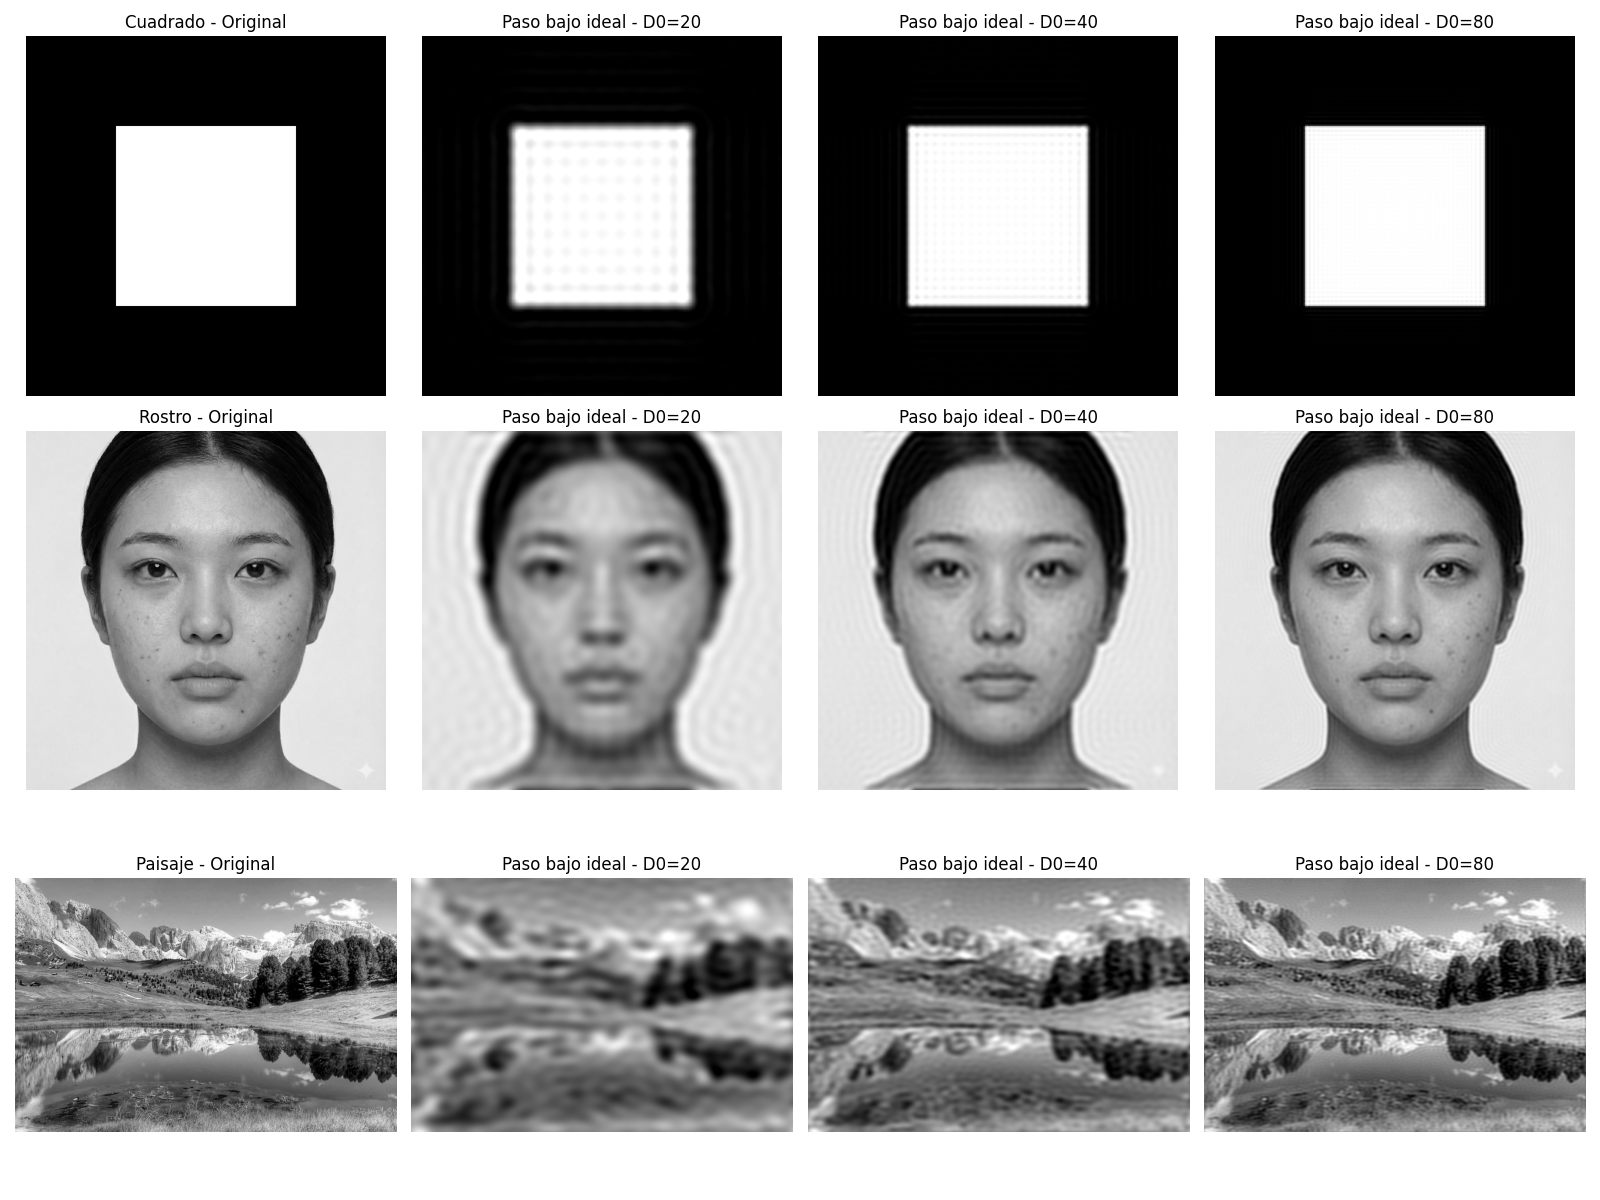
\includegraphics[width=\textwidth]
    {../results/filtro_ideal_paso_bajo.png}
    \caption{Filtro ideal paso bajo con
    frecuencias de corte de 20, 40 y 80.}
    \label{fig:ideal_lp}
\end{figure}

En el cuadrado, el corte de 20 produce
un suavizado evidente y aparecen halos
alrededor de los contornos. Al aumentar
la frecuencia de corte, los bordes
recuperan definición y las oscilaciones
son menos visibles.

En el rostro se reducen las pequeñas
variaciones de intensidad de la piel,
pero también se pierde definición en
los ojos, las cejas y el cabello.
Se observan algunas bandas alrededor
de la silueta.

En el paisaje, el corte de 20 elimina
numerosos detalles de montañas, árboles
y reflejos. Los cortes de 40 y 80
conservan progresivamente más texturas.

Estos resultados muestran que el filtro
ideal suaviza al eliminar frecuencias altas,
pero puede introducir el efecto de anillado
(\textit{ringing}) debido a su corte abrupto.

% ---------------------------------------------------------
\subsection{Punto 2: Filtro Butterworth paso bajo}

\subsubsection*{Objetivo}

Implementar un filtro Butterworth paso bajo
que reciba la imagen, la frecuencia de corte
y el orden del filtro.

\subsubsection*{Fundamento}

A diferencia del filtro ideal, Butterworth
atenúa las frecuencias de forma gradual:

\begin{equation}
H(u,v)=
\frac{1}{
1+\left(
\frac{D(u,v)}{D_0}
\right)^{2n}
}
\end{equation}

El parámetro $n$ representa el orden.

Cuanto mayor es el orden, más abrupta
se vuelve la transición entre frecuencias.

Con esta formulación, la ganancia en
$D(u,v)=D_0$ es igual a 0,5,
independientemente del orden.

\subsubsection*{Implementación}

\begin{lstlisting}
def filtro_butterworth_paso_bajo(
    imagen, frecuencia_corte, orden
):

    if frecuencia_corte <= 0:
        raise ValueError(
            "La frecuencia de corte debe ser positiva"
        )

    if orden <= 0 or int(orden) != orden:
        raise ValueError(
            "El orden debe ser un entero positivo"
        )

    filas, columnas = imagen.shape

    mascara = np.zeros(
        (filas, columnas),
        dtype=np.float64
    )

    centro_fila = filas // 2
    centro_columna = columnas // 2

    for fila in range(filas):
        for columna in range(columnas):

            distancia = np.sqrt(
                (fila - centro_fila)**2
                + (columna - centro_columna)**2
            )

            mascara[fila, columna] = 1 / (
                1 + (
                    distancia / frecuencia_corte
                )**(2 * orden)
            )

    transformada = np.fft.fft2(imagen)
    transformada_centrada = np.fft.fftshift(
        transformada
    )
    transformada_filtrada = (
        transformada_centrada * mascara
    )
    transformada_inversa = np.fft.ifftshift(
        transformada_filtrada
    )
    imagen_filtrada = np.fft.ifft2(
        transformada_inversa
    )
    resultado = np.real(imagen_filtrada)

    return resultado, mascara
\end{lstlisting}

\subsubsection*{Resultados y análisis}

Se realizaron dos pruebas: variación de
la frecuencia de corte con orden 2 y
variación del orden manteniendo $D_0=40$.

\begin{figure}[H]
    \centering
    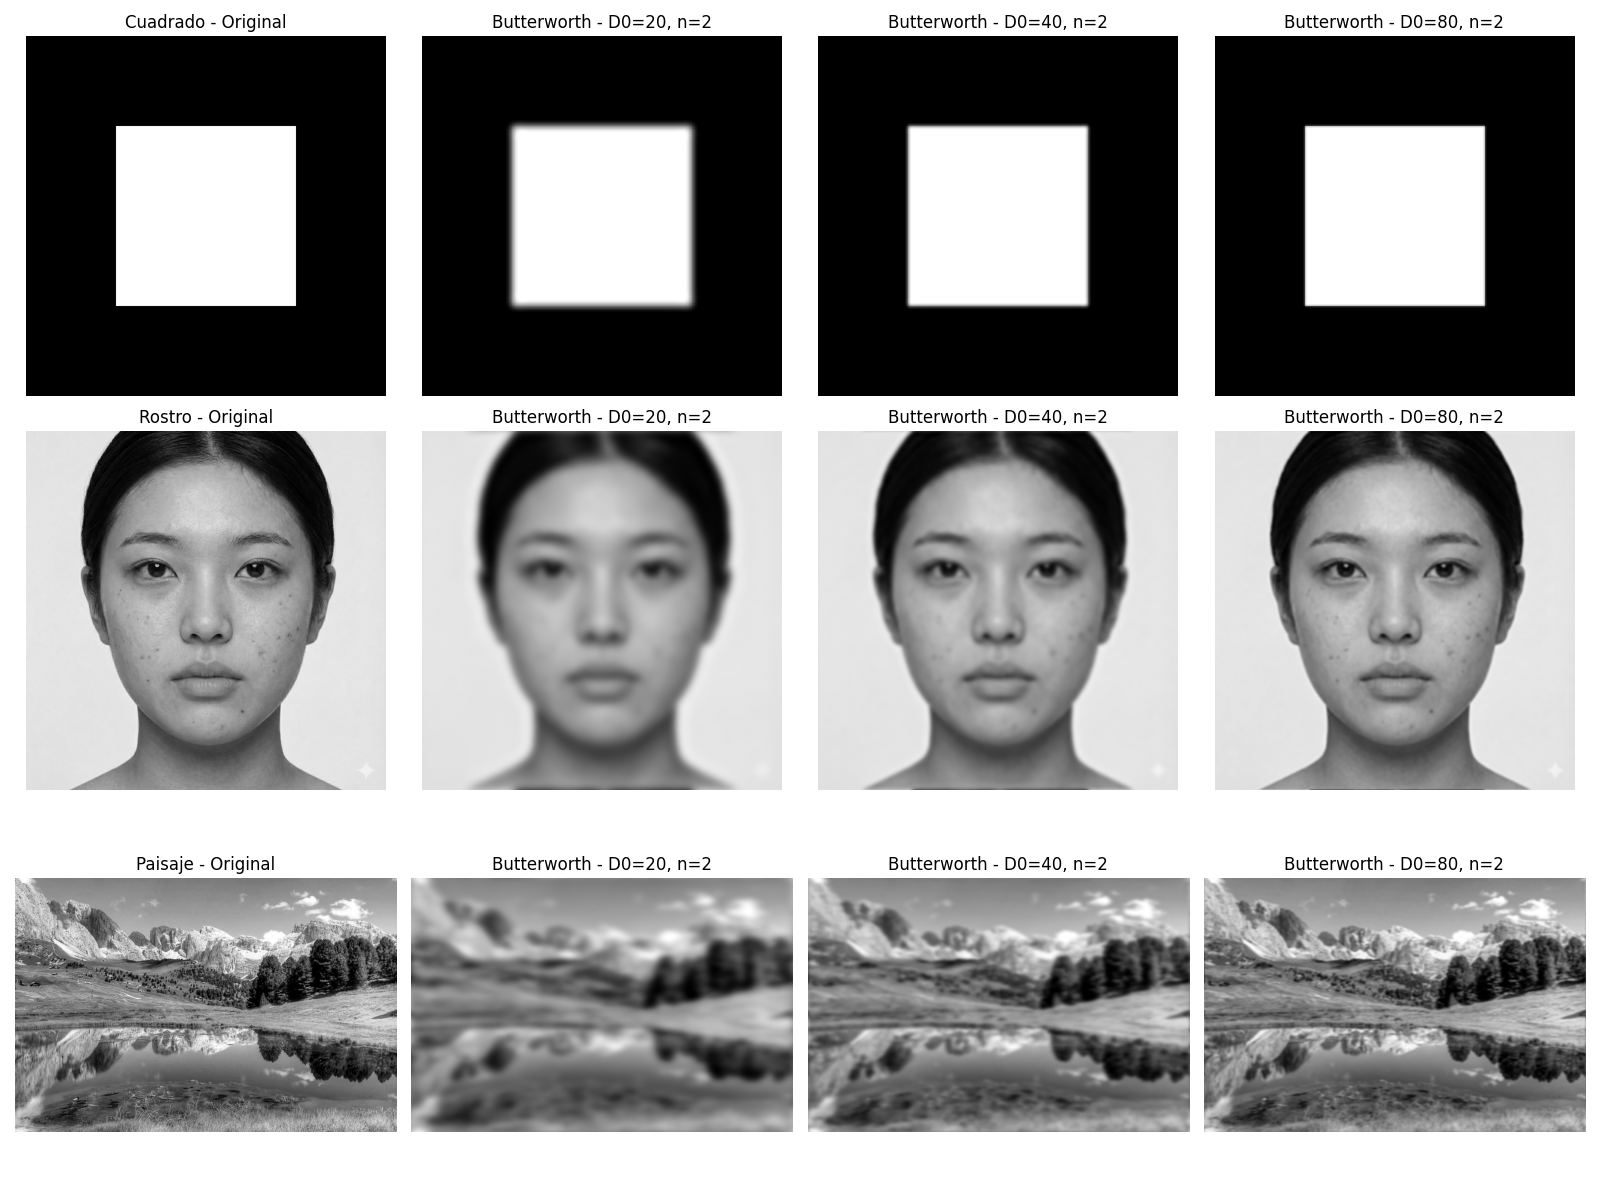
\includegraphics[width=\textwidth]
    {../results/filtro_butterworth_paso_bajo.png}
    \caption{Butterworth paso bajo con
    $D_0=20$, 40 y 80, y orden 2.}
    \label{fig:butter_lp_corte}
\end{figure}

Con $D_0=20$ se observa un suavizado
considerable en las tres imágenes.
Al aumentar la frecuencia de corte,
se recuperan progresivamente detalles
del cuadrado, el rostro y el paisaje.

Los bordes presentan menos oscilaciones
pronunciadas que con el filtro ideal.

\begin{figure}[H]
    \centering
    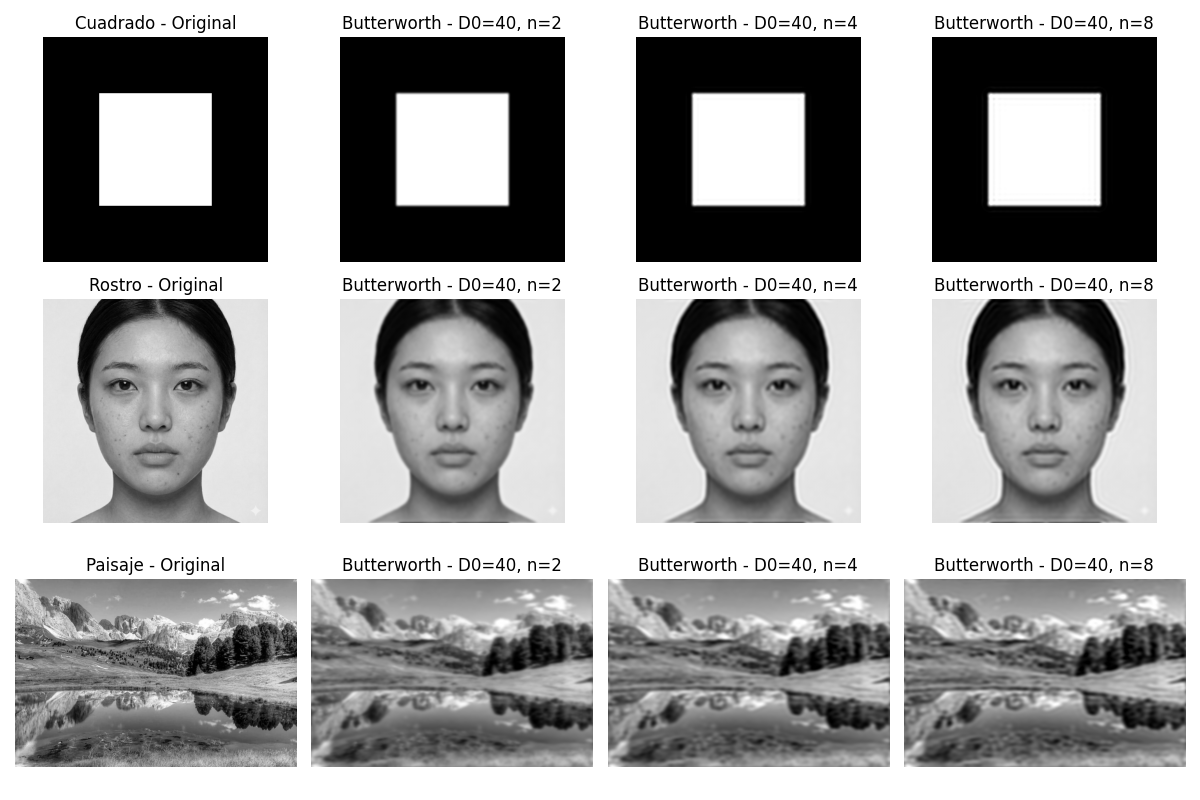
\includegraphics[width=\textwidth]
    {../results/filtro_butterworth_varios_ordenes.png}
    \caption{Butterworth paso bajo con
    $D_0=40$ y órdenes 2, 4 y 8.}
    \label{fig:butter_lp_orden}
\end{figure}

Al aumentar el orden, los cambios visuales
son más sutiles que al modificar la
frecuencia de corte.

En el cuadrado, el orden 8 produce
pequeñas oscilaciones cerca de los bordes.
En el rostro también aparecen algunas
bandas alrededor de la silueta.

En el paisaje se observan variaciones
leves en la definición de montañas,
árboles y reflejos.

Esto confirma que Butterworth permite
controlar el suavizado mediante dos
parámetros distintos: el corte determina
la región de transición y el orden
determina su brusquedad.

% ---------------------------------------------------------
\subsection{Punto 3: Filtro Gaussiano paso bajo}

\subsubsection*{Objetivo}

Implementar mediante ciclos un filtro
Gaussiano paso bajo en 2D utilizando
la imagen y la frecuencia de corte.

\subsubsection*{Fundamento}

El filtro Gaussiano paso bajo utiliza:

\begin{equation}
H(u,v)=
e^{-\frac{D^2(u,v)}{2D_0^2}}
\end{equation}

Atenúa progresivamente las frecuencias
altas sin establecer una frontera abrupta.

A diferencia de Butterworth, no utiliza
un parámetro de orden.

\subsubsection*{Implementación}

\begin{lstlisting}
def filtro_gaussiano_paso_bajo(
    imagen, frecuencia_corte
):

    if frecuencia_corte <= 0:
        raise ValueError(
            "La frecuencia de corte debe ser positiva"
        )

    filas, columnas = imagen.shape

    mascara = np.zeros(
        (filas, columnas),
        dtype=np.float64
    )

    centro_fila = filas // 2
    centro_columna = columnas // 2

    for fila in range(filas):
        for columna in range(columnas):

            distancia = np.sqrt(
                (fila - centro_fila)**2
                + (columna - centro_columna)**2
            )

            mascara[fila, columna] = np.exp(
                -(distancia**2) /
                (2 * frecuencia_corte**2)
            )

    transformada = np.fft.fft2(imagen)
    transformada_centrada = np.fft.fftshift(
        transformada
    )
    transformada_filtrada = (
        transformada_centrada * mascara
    )
    transformada_inversa = np.fft.ifftshift(
        transformada_filtrada
    )
    imagen_filtrada = np.fft.ifft2(
        transformada_inversa
    )
    resultado = np.real(imagen_filtrada)

    return resultado, mascara
\end{lstlisting}

\subsubsection*{Resultados y análisis}

\begin{figure}[H]
    \centering
    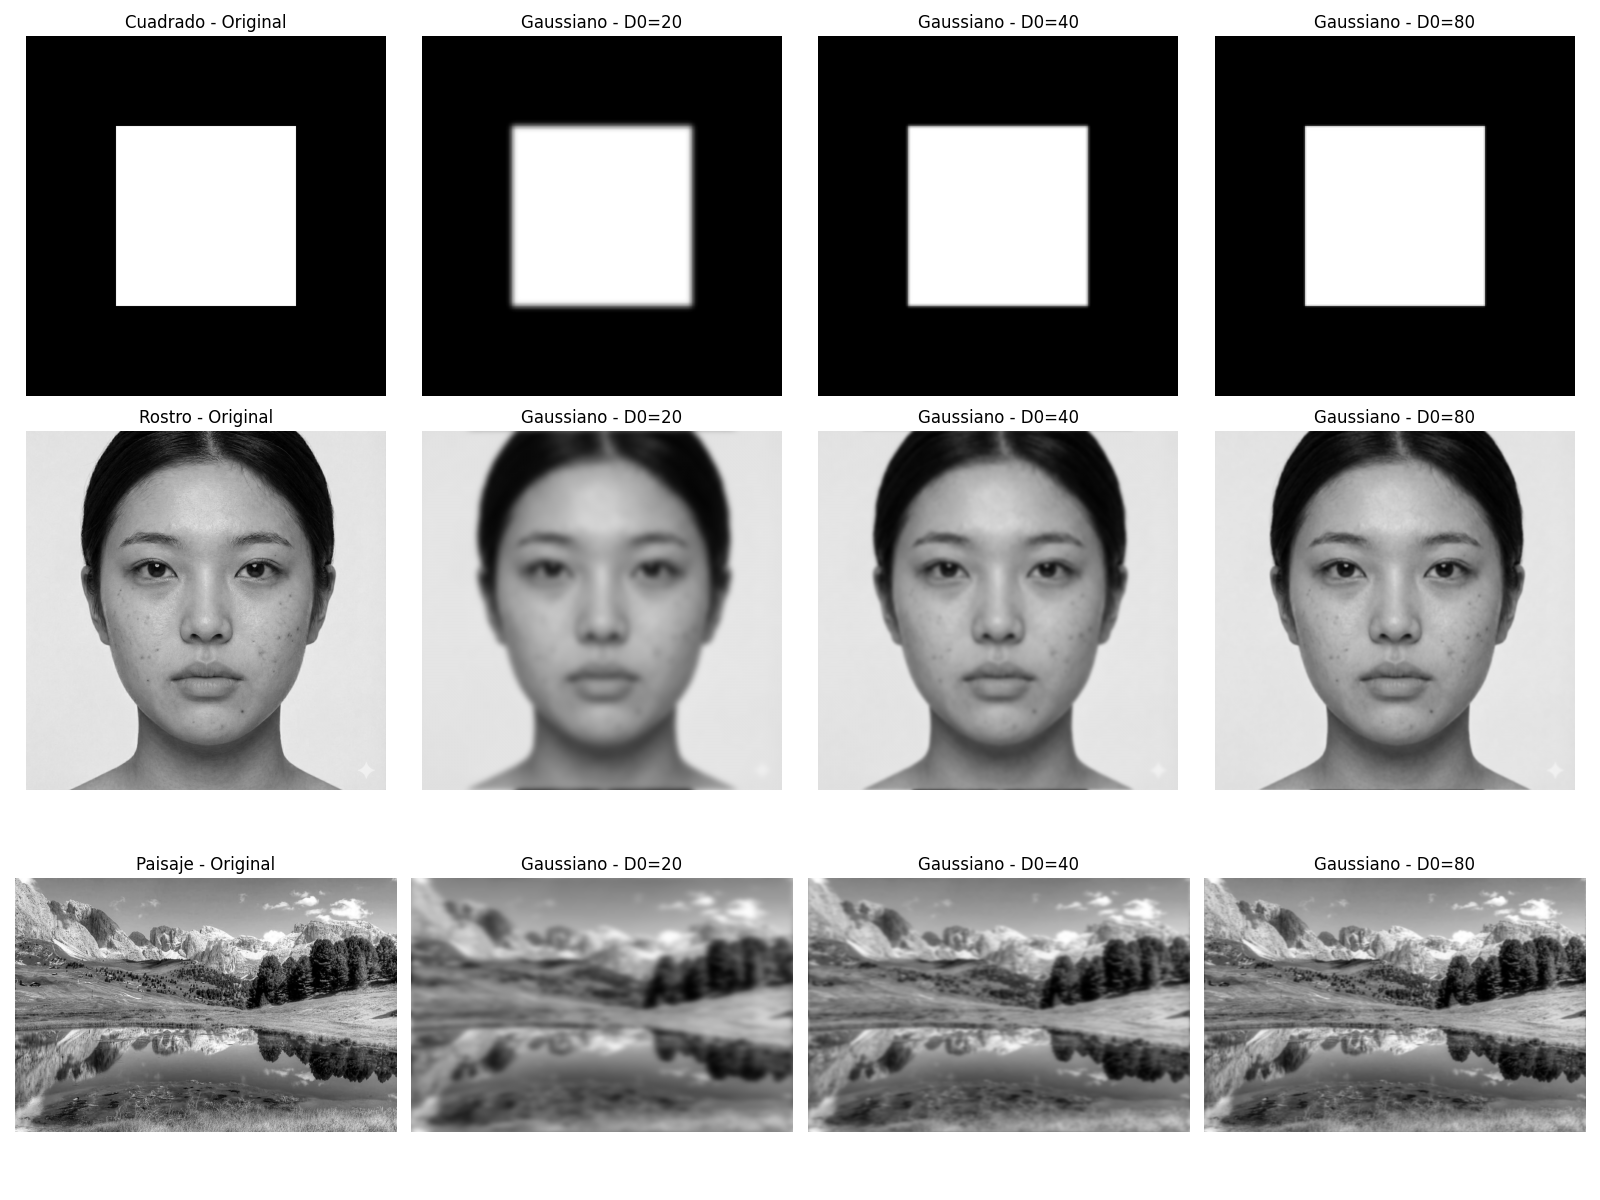
\includegraphics[width=\textwidth]
    {../results/filtro_gaussiano_paso_bajo.png}
    \caption{Filtro Gaussiano paso bajo
    con frecuencias de corte de 20, 40 y 80.}
    \label{fig:gauss_lp}
\end{figure}

Con $D_0=20$, el cuadrado presenta
bordes suavizados, mientras que el
rostro y el paisaje pierden detalles finos.

Al utilizar cortes de 40 y 80, las
imágenes recuperan gradualmente
su definición.

Las transiciones son suaves y no
se aprecian oscilaciones pronunciadas
alrededor de los contornos.

Los resultados muestran que el
Gaussiano produce un suavizado gradual,
aunque una atenuación intensa también
puede eliminar detalles importantes.

% =========================================================
\section{Filtros paso alto}

Los tres ejercicios restantes utilizan
máscaras que atenúan las frecuencias bajas
y conservan progresivamente las altas.

Para construirlas se empleó la relación:

\[
H_{HP}(u,v)=1-H_{LP}(u,v)
\]

La visualización de los resultados se realizó
mediante \texttt{np.abs()}, debido a que
la transformada inversa puede producir
respuestas reales positivas y negativas.

Se mantuvo una escala visual fija de
0 a 255 para facilitar la comparación.

% ---------------------------------------------------------
\subsection{Punto 4: Filtro ideal paso alto}

\subsubsection*{Objetivo}

Implementar un filtro ideal paso alto
en 2D que reciba la imagen original
y la frecuencia de corte.

\subsubsection*{Fundamento}

Su función de transferencia es:

\begin{equation}
H(u,v)=
\begin{cases}
0, & D(u,v)\leq D_0\\
1, & D(u,v)>D_0
\end{cases}
\end{equation}

Las frecuencias cercanas al centro
se eliminan, mientras que las
más alejadas se conservan.

\subsubsection*{Implementación}

\begin{lstlisting}
def filtro_ideal_paso_alto(
    imagen, frecuencia_corte
):

    if frecuencia_corte <= 0:
        raise ValueError(
            "La frecuencia de corte debe ser positiva"
        )

    filas, columnas = imagen.shape

    mascara = np.ones(
        (filas, columnas),
        dtype=np.float64
    )

    centro_fila = filas // 2
    centro_columna = columnas // 2

    for fila in range(filas):
        for columna in range(columnas):

            distancia = np.sqrt(
                (fila - centro_fila)**2
                + (columna - centro_columna)**2
            )

            if distancia <= frecuencia_corte:
                mascara[fila, columna] = 0

    transformada = np.fft.fft2(imagen)
    transformada_centrada = np.fft.fftshift(
        transformada
    )
    transformada_filtrada = (
        transformada_centrada * mascara
    )
    transformada_inversa = np.fft.ifftshift(
        transformada_filtrada
    )
    imagen_filtrada = np.fft.ifft2(
        transformada_inversa
    )
    resultado = np.real(imagen_filtrada)

    return resultado, mascara
\end{lstlisting}

\subsubsection*{Resultados y análisis}

\begin{figure}[H]
    \centering
    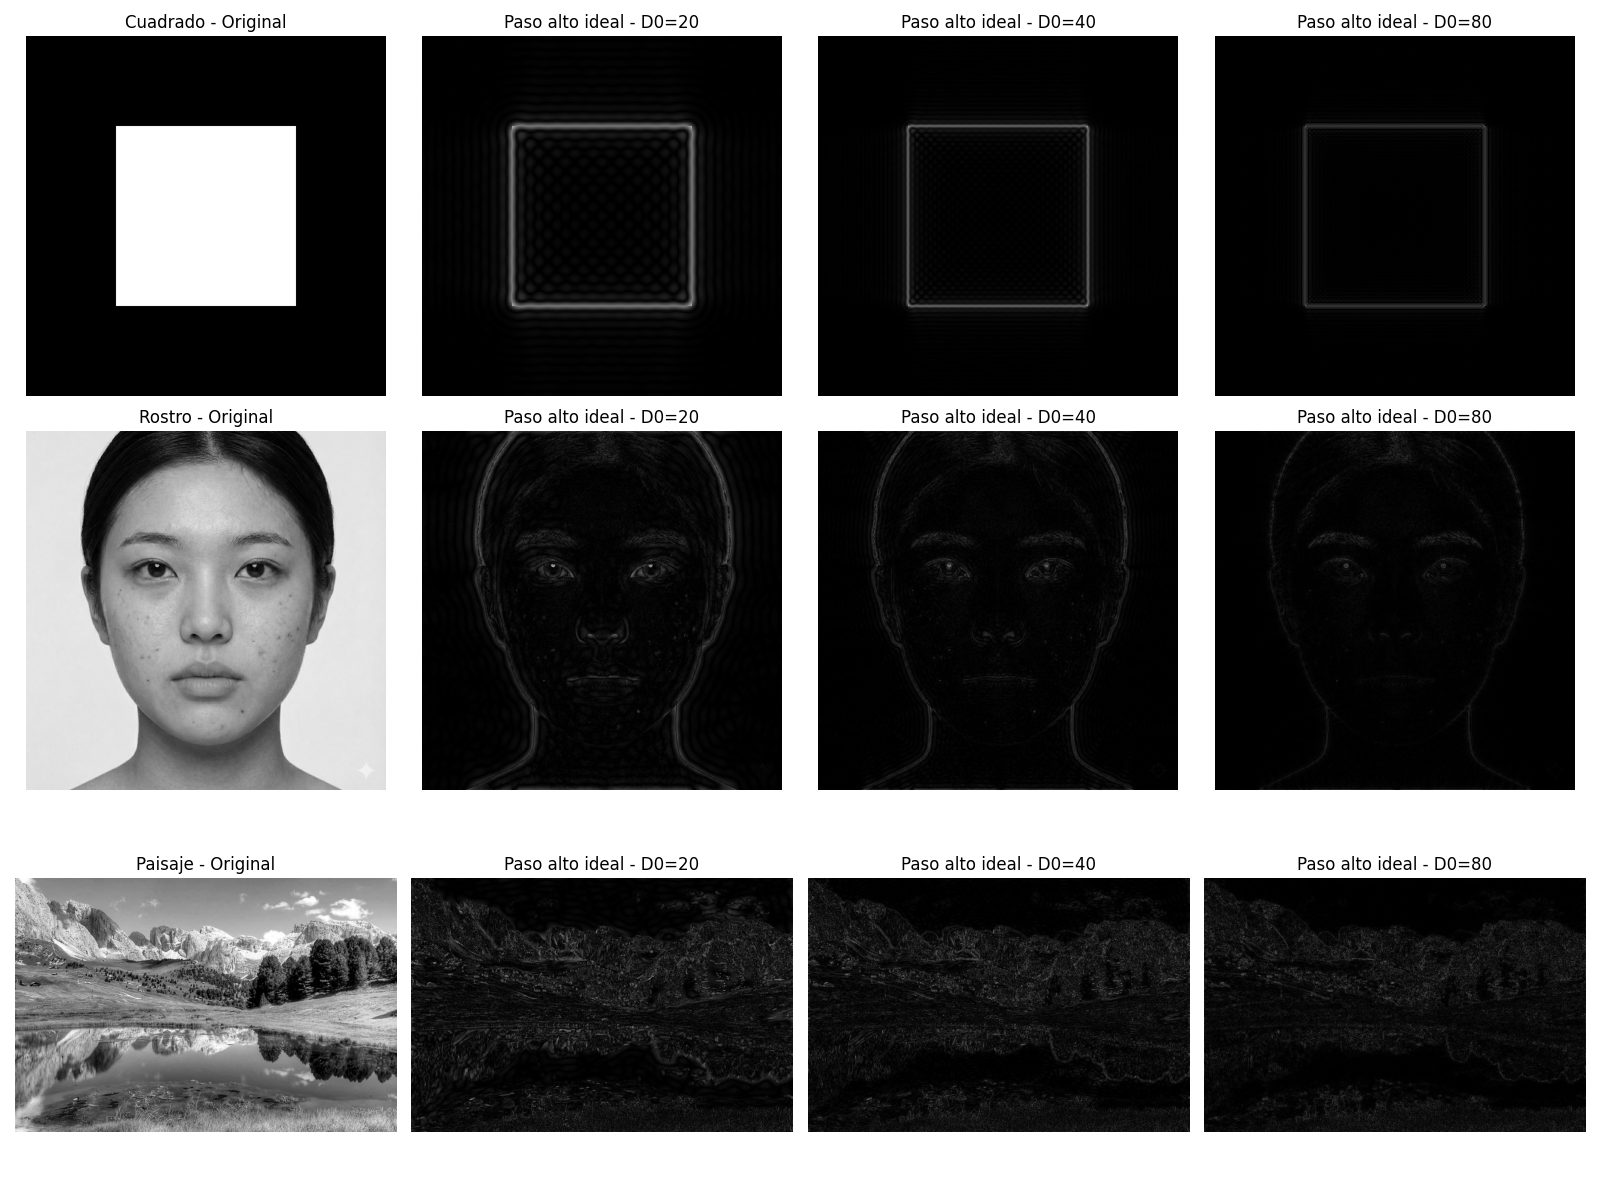
\includegraphics[width=\textwidth]
    {../results/filtro_ideal_paso_alto.png}
    \caption{Filtro ideal paso alto con
    frecuencias de corte de 20, 40 y 80.}
    \label{fig:ideal_hp}
\end{figure}

En el cuadrado, el corte de 20 permite
visualizar claramente sus contornos,
acompañados de oscilaciones dentro
y alrededor de la figura.

Con cortes de 40 y 80, los contornos
aparecen progresivamente más tenues.

En el rostro se destacan los ojos,
el cabello, los labios y la silueta,
mientras que en el paisaje aparecen
bordes de montañas, árboles y reflejos.

Al aumentar la frecuencia de corte,
las respuestas se vuelven menos visibles,
porque se elimina una región cada vez
mayor del espectro.

El filtro ideal paso alto destaca
las variaciones rápidas de intensidad,
pero su corte abrupto puede producir
anillado alrededor de los bordes.

% ---------------------------------------------------------
\subsection{Punto 5: Filtro Butterworth paso alto}

\subsubsection*{Objetivo}

Implementar un filtro Butterworth paso alto
en 2D que reciba la imagen, la frecuencia
de corte y el orden.

\subsubsection*{Fundamento}

Se obtiene mediante el complemento
del filtro Butterworth paso bajo:

\begin{equation}
H_{HP}(u,v)=
1-
\frac{1}{
1+\left(
\frac{D(u,v)}{D_0}
\right)^{2n}
}
\end{equation}

La frecuencia de corte determina
la región de atenuación, mientras que
el orden controla la brusquedad
de la transición.

\subsubsection*{Implementación}

\begin{lstlisting}
def filtro_butterworth_paso_alto(
    imagen, frecuencia_corte, orden
):

    if frecuencia_corte <= 0:
        raise ValueError(
            "La frecuencia de corte debe ser positiva"
        )

    if orden <= 0 or int(orden) != orden:
        raise ValueError(
            "El orden debe ser un entero positivo"
        )

    filas, columnas = imagen.shape

    mascara = np.zeros(
        (filas, columnas),
        dtype=np.float64
    )

    centro_fila = filas // 2
    centro_columna = columnas // 2

    for fila in range(filas):
        for columna in range(columnas):

            distancia = np.sqrt(
                (fila - centro_fila)**2
                + (columna - centro_columna)**2
            )

            paso_bajo = 1 / (
                1 + (
                    distancia / frecuencia_corte
                )**(2 * orden)
            )

            mascara[fila, columna] = 1 - paso_bajo

    transformada = np.fft.fft2(imagen)
    transformada_centrada = np.fft.fftshift(
        transformada
    )
    transformada_filtrada = (
        transformada_centrada * mascara
    )
    transformada_inversa = np.fft.ifftshift(
        transformada_filtrada
    )
    imagen_filtrada = np.fft.ifft2(
        transformada_inversa
    )
    resultado = np.real(imagen_filtrada)

    return resultado, mascara
\end{lstlisting}

\subsubsection*{Resultados y análisis}

Primero se compararon las frecuencias
de corte 20, 40 y 80 con orden 2.

\begin{figure}[H]
    \centering
    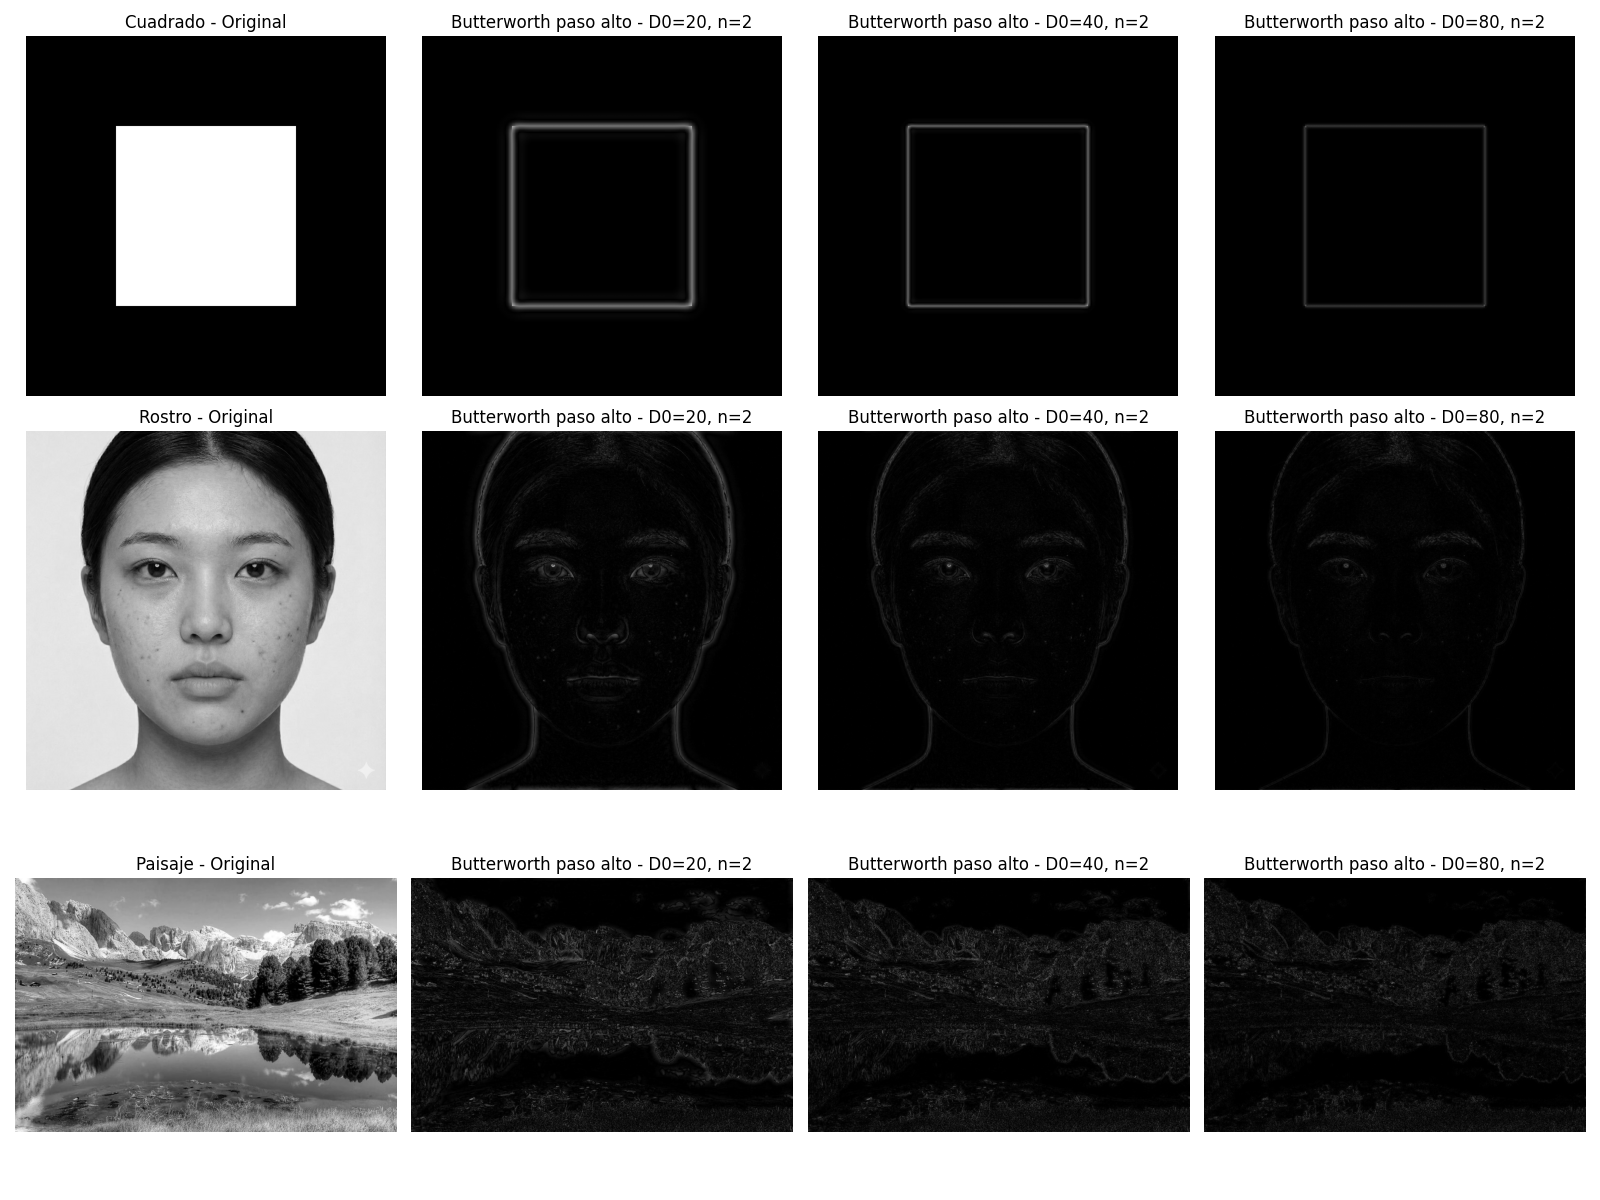
\includegraphics[width=\textwidth]
    {../results/filtro_butterworth_paso_alto.png}
    \caption{Butterworth paso alto con
    cortes 20, 40 y 80, y orden 2.}
    \label{fig:butter_hp_corte}
\end{figure}

Con el corte de 20 aparecen claramente
los contornos del cuadrado, del rostro
y de las estructuras del paisaje.

A medida que aumenta la frecuencia
de corte, las respuestas se vuelven
más tenues y las imágenes más oscuras.

En el cuadrado se observan contornos
más uniformes que con el filtro ideal,
sin tantas oscilaciones alrededor.

Posteriormente se mantuvo $D_0=40$
y se utilizaron órdenes 2, 4 y 8.

\begin{figure}[H]
    \centering
    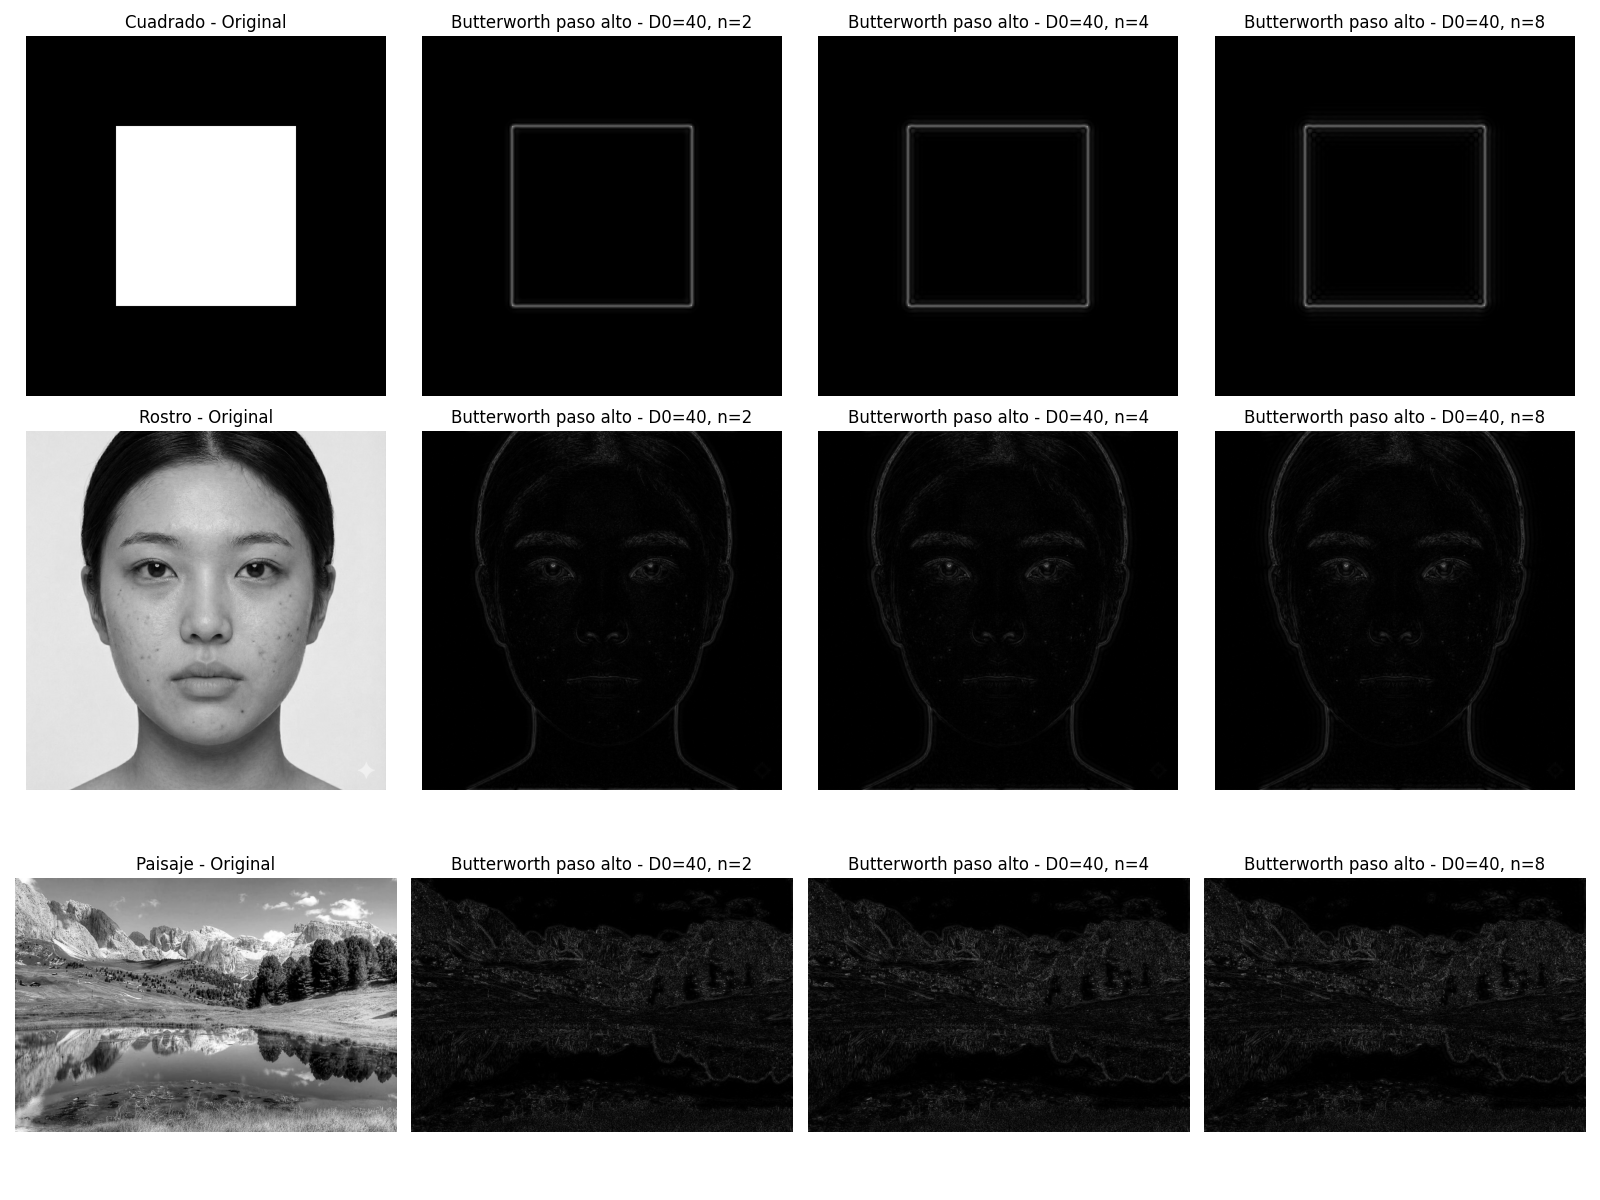
\includegraphics[width=\textwidth]
    {../results/filtro_butterworth_paso_alto_ordenes.png}
    \caption{Butterworth paso alto con
    $D_0=40$ y órdenes 2, 4 y 8.}
    \label{fig:butter_hp_orden}
\end{figure}

En las imágenes completas, las diferencias
entre órdenes son relativamente pequeñas.

En el paisaje, con orden 8, algunos bordes
de montañas y árboles parecen ligeramente
más definidos.

Para estudiar mejor este comportamiento
se amplió una esquina del cuadrado.

\begin{figure}[H]
    \centering
    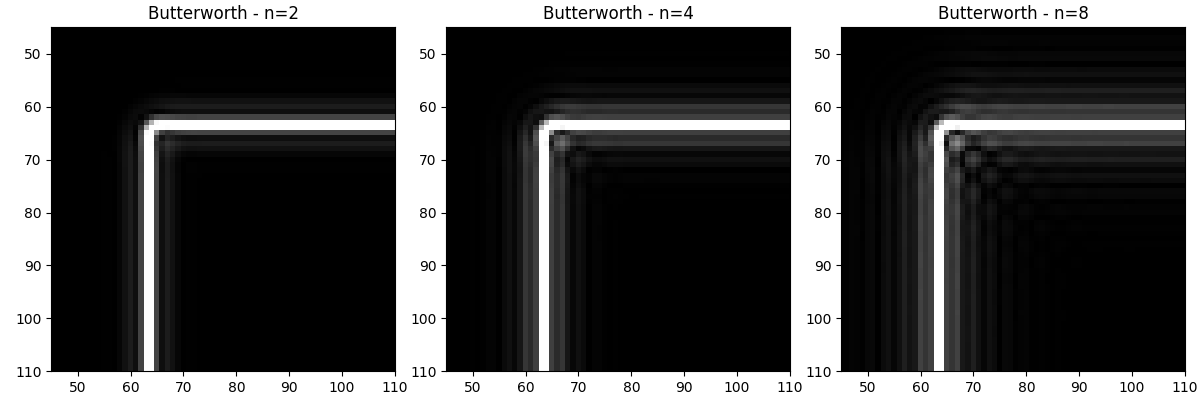
\includegraphics[width=\textwidth]
    {../results/filtro_butterworth_paso_alto_zoom.png}
    \caption{Ampliación de una esquina del cuadrado
    para comparar los órdenes 2, 4 y 8.}
    \label{fig:butter_hp_zoom}
\end{figure}

La ampliación permite identificar
diferencias que no eran evidentes
en las imágenes completas.

Con orden 2, los bordes son suaves
y relativamente uniformes.

Con orden 4 aparecen pequeñas líneas
adicionales, mientras que con orden 8
las oscilaciones son mucho más visibles,
especialmente dentro del cuadrado.

Esto sucede porque un orden mayor
produce una transición más abrupta,
aproximándose al comportamiento ideal.

Por tanto, aumentar el orden no implica
necesariamente una mejor detección
de bordes, ya que también puede
introducir artefactos.

% ---------------------------------------------------------
\subsection{Punto 6: Filtro Gaussiano paso alto}

\subsubsection*{Objetivo}

Implementar mediante ciclos un filtro
Gaussiano paso alto que reciba la imagen
original y la frecuencia de corte.

\subsubsection*{Fundamento}

El Gaussiano paso alto se define como:

\begin{equation}
H_{HP}(u,v)=
1-e^{-\frac{D^2(u,v)}{2D_0^2}}
\end{equation}

Elimina la componente de frecuencia cero
y conserva progresivamente las componentes
más altas.

Su transición suave permite evitar
las discontinuidades propias
del filtro ideal.

\subsubsection*{Implementación}

\begin{lstlisting}
def filtro_gaussiano_paso_alto(
    imagen, frecuencia_corte
):

    if frecuencia_corte <= 0:
        raise ValueError(
            "La frecuencia de corte debe ser positiva"
        )

    filas, columnas = imagen.shape

    mascara = np.zeros(
        (filas, columnas),
        dtype=np.float64
    )

    centro_fila = filas // 2
    centro_columna = columnas // 2

    for fila in range(filas):
        for columna in range(columnas):

            distancia = np.sqrt(
                (fila - centro_fila)**2
                + (columna - centro_columna)**2
            )

            paso_bajo = np.exp(
                -(distancia**2) /
                (2 * frecuencia_corte**2)
            )

            mascara[fila, columna] = 1 - paso_bajo

    transformada = np.fft.fft2(imagen)
    transformada_centrada = np.fft.fftshift(
        transformada
    )
    transformada_filtrada = (
        transformada_centrada * mascara
    )
    transformada_inversa = np.fft.ifftshift(
        transformada_filtrada
    )
    imagen_filtrada = np.fft.ifft2(
        transformada_inversa
    )
    resultado = np.real(imagen_filtrada)

    return resultado, mascara
\end{lstlisting}

\subsubsection*{Resultados y análisis}

\begin{figure}[H]
    \centering
    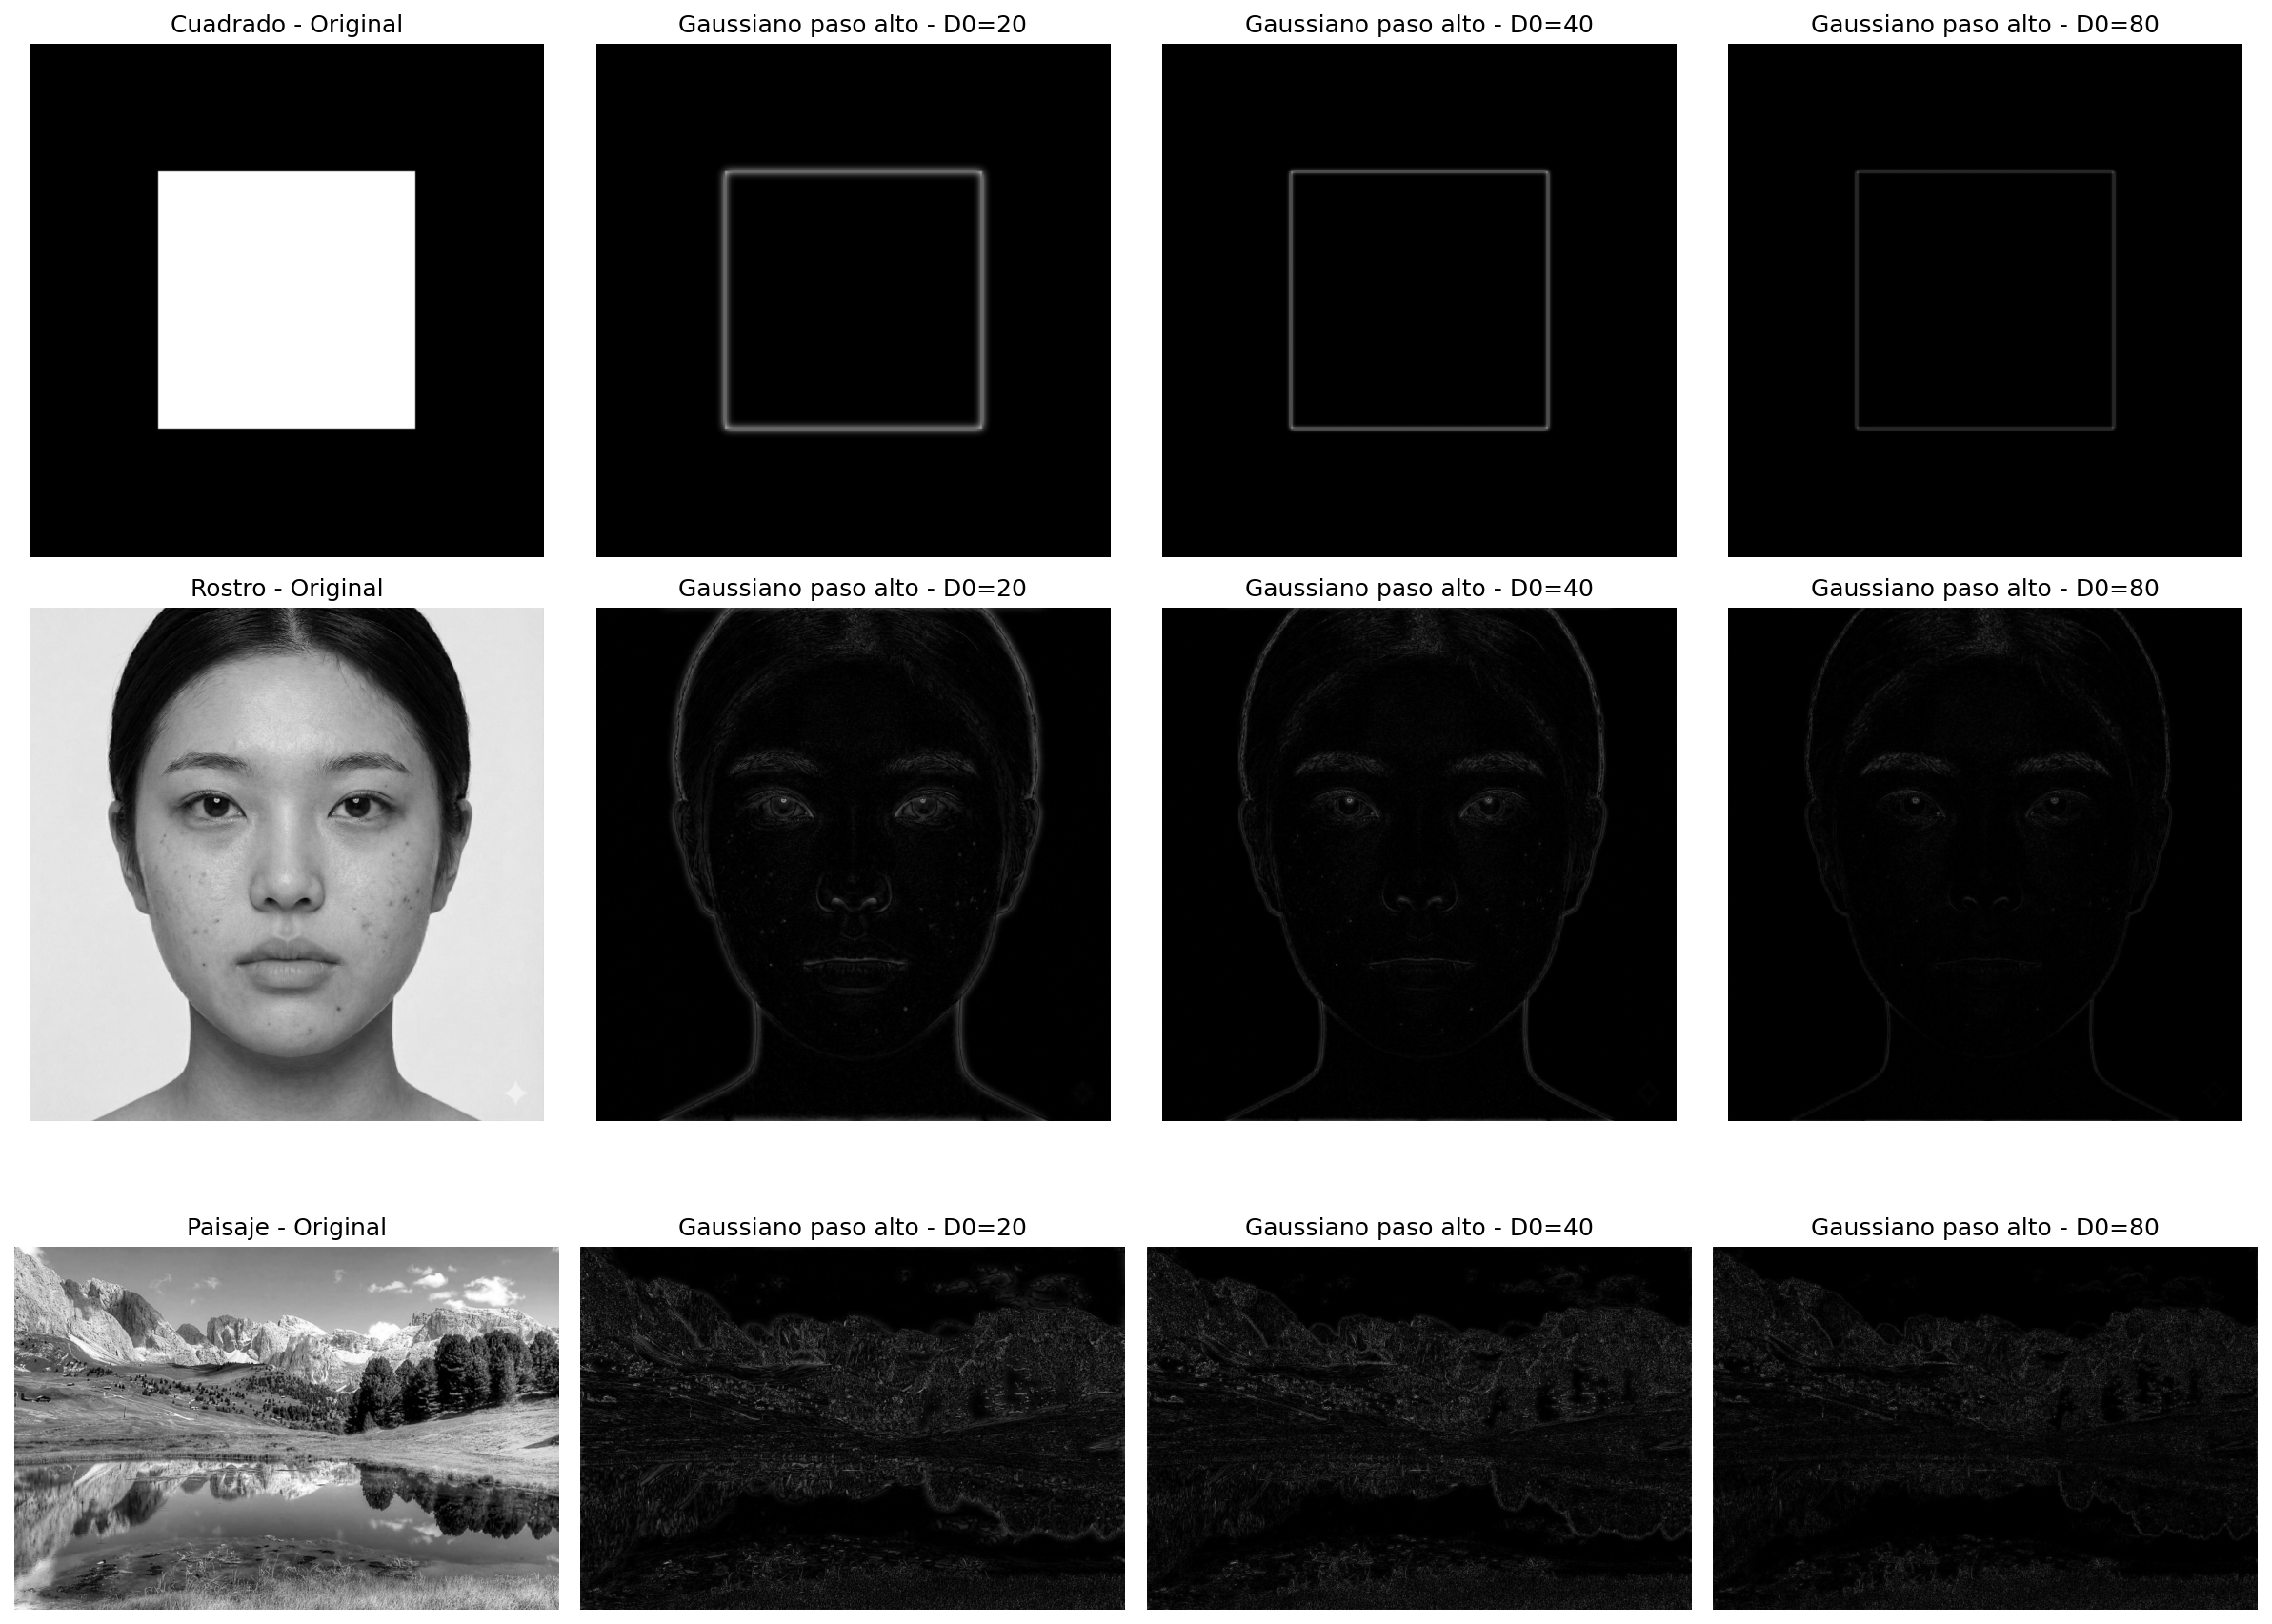
\includegraphics[width=\textwidth]
    {../results/filtro_gaussiano_paso_alto.png}
    \caption{Filtro Gaussiano paso alto
    con frecuencias de corte de 20, 40 y 80.}
    \label{fig:gauss_hp}
\end{figure}

En el cuadrado, el corte de 20 produce
contornos relativamente gruesos y brillantes.

Al aumentar la frecuencia de corte a
40 y 80, las respuestas se vuelven
más finas y tenues.

Este comportamiento también se aprecia
en el rostro, donde los contornos de
ojos, nariz, labios y cabello pierden
intensidad visual al aumentar el corte.

En el paisaje se destacan montañas,
árboles, vegetación y reflejos.
Con cortes mayores, permanecen visibles
principalmente variaciones más finas.

En las tres imágenes se observan
contornos relativamente uniformes,
sin oscilaciones pronunciadas.

Estos resultados muestran que el Gaussiano
paso alto permite destacar variaciones
rápidas de intensidad mediante
una transición gradual de frecuencias.

% =========================================================
\section{Análisis general}

Los resultados permiten comprender
que el efecto de un filtro depende
de qué frecuencias conserva y cuáles
atenúa, además de la forma de transición
de su máscara.

En los filtros paso bajo, las frecuencias
de corte menores produjeron un suavizado
más intenso, especialmente visible
en los detalles del rostro y del paisaje.

Al aumentar el corte, se conservaron
progresivamente más texturas y contornos.

En los filtros paso alto se observó
el comportamiento contrario:
se destacaron principalmente los bordes
y las variaciones rápidas de intensidad.

Con la escala visual utilizada, aumentar
el corte hizo que muchas respuestas
fueran más débiles y menos visibles.

También se identificaron diferencias
entre las tres familias de filtros.

El filtro ideal realizó cortes abruptos
y produjo oscilaciones alrededor de
algunos bordes.

Butterworth permitió controlar
la transición mediante el orden.
La ampliación del cuadrado demostró
que los órdenes altos pueden producir
un anillado más pronunciado.

Por su parte, el filtro Gaussiano
presentó transiciones suaves,
sin oscilaciones evidentes de la
misma intensidad que las observadas
con el filtro ideal.

Las tres imágenes resultaron útiles
para estudiar diferentes aspectos
del procesamiento.

El cuadrado facilitó la identificación
de halos y cambios en los contornos.

El rostro permitió observar el efecto
sobre texturas pequeñas y rasgos faciales.

El paisaje permitió analizar
la conservación o pérdida de detalles
en estructuras naturales.

En conjunto, los resultados mostraron
que no existe un filtro universalmente
mejor, sino que su selección depende
del propósito del procesamiento
y de las características de la imagen.

% =========================================================
\section{Conclusiones}

Se implementaron correctamente seis filtros
en el dominio de la frecuencia utilizando
máscaras construidas mediante ciclos
y transformaciones de Fourier.

Los filtros paso bajo permitieron suavizar
las imágenes al atenuar las frecuencias
altas. Los resultados también mostraron
que un suavizado intenso puede eliminar
detalles importantes.

Los filtros paso alto permitieron destacar
bordes y texturas al reducir la contribución
de las frecuencias bajas.

La frecuencia de corte fue un parámetro
fundamental en ambos tipos de filtrado,
ya que determinó las componentes que
se conservaron o atenuaron.

La comparación entre las familias
permitió observar que los filtros ideales
pueden generar oscilaciones debido
a su corte abrupto.

Butterworth ofreció una transición
controlable, aunque los órdenes altos
también favorecieron la aparición
de anillado, como se comprobó
en la ampliación del cuadrado.

Finalmente, el filtro Gaussiano mostró
un comportamiento gradual y resultados
sin oscilaciones pronunciadas,
aunque también modificó la definición
de los detalles.

En general, el taller permitió relacionar
los conceptos de
\textbf{frecuencia espacial, FFT,
máscaras de filtrado, frecuencia de corte,
orden y reconstrucción de imágenes},
comprendiendo cómo estos elementos
influyen en los resultados del procesamiento.

\end{document}
